% This file should be compiled as such: PdfLatex -> Bibtex -> PdfLatex (x2)

\documentclass[parskip=full-]{scrreprt}

\KOMAoptions{numbers=noendperiod}

\usepackage{chngcntr}
\counterwithout{figure}{chapter}

\usepackage[utf8]{inputenc}

\usepackage{amsmath}
\newcommand\Rey{\mathrm{Re}}

\usepackage{amsfonts}
\usepackage{amssymb}
\usepackage{outlines}
\usepackage{xcolor}
\usepackage{geometry}
\usepackage{siunitx}

\usepackage{marginnote}
\renewcommand*{\marginfont}{\color{red}\sffamily}

\usepackage{lineno}
\renewcommand\linenumberfont{\normalfont\small\sffamily}
\linenumbers

\usepackage{graphicx}
\graphicspath{{../pics/}}

\usepackage{natbib}

\author{Jordan Wingenroth, Candace Yee, Justin Nghiem, and Laurel Larsen}

\title{Effective collector efficiency of sparse and dense arrays of emergent cylindrical collectors in laminar-turbulent transitional flows}

\begin{document}

\maketitle

\chapter{Introduction}

TODO

\chapter{Methods}

\section{Theoretical Background}

In this study, we focus on direct interception of suspended particles by submerged vegetation. Direct interception is the adhesion of particles traveling along streamlines to the surfaces of collectors (e.g., plants). This is just one of several fluid dynamics mechanisms that act on suspended particles. Others include gravitational settling, inertial impaction, and diffusional deposition. Gravitational settling is the process of particles denser than water being drawn towards and coming to rest on the channel bottom. Inertial impaction and diffusional deposition are other means by which suspended particles can adhere to collectors. Inertial impaction occurs when particles possess momentum relative to streamlines, and diffusional deposition arises due to some combination of turbulence and Brownian motion.

Capture efficiency ($\eta=\frac{b_c}{d_c}$) is defined as the ratio between the upstream width ($b_c$) of the streamlines that encounter a collector and the collector's own diameter (\(d_c\)), which may be represented by an effective diameter in the case of non-cylindrical collectors (Figure \ref{fig:capeff}). Effective particle capture efficiency (\(\eta\prime=p_r\frac{b_c}{d_c}\)) takes into account the fact that not all particles coming into contact with a collector will adhere to it, thus including probability of retention (\(p_r\)) as a multiplicand in its calculation. This parameter, as opposed to theoretical capture efficiency $\eta$, corresponds to the empirical estimates made by our study, and presumably any others that leave $p_r$ as an implicit factor.

\begin{figure}[htbp]
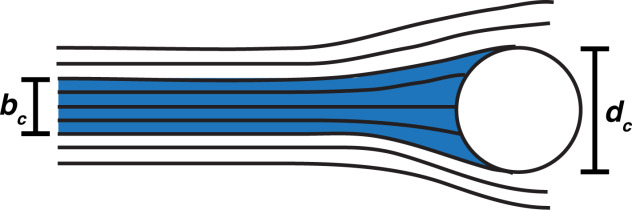
\includegraphics[width=10cm]{fauria particle capture efficiency diagram.jpg}
\centering
\caption[xxx]{Particle capture efficiency diagram (TODO: caption) \label{fig:capeff}
\end{figure}

Particle capture in transitionally turbulent flows (\(1<\Rey<1000\)), which occur commonly in the environments and on the length scales of aquatic macrovegetation, does not follow the analytical expressions involving Reynolds number, collector diameter, and particle diameter (\(d_p\)), derived for creeping flow. Hence, empirical estimates must be used. \citet{Palmer_2004} introduced a power law expression for estimating capture efficiency of cylindrical collectors, which takes the form \[\eta=C{\Rey_c}^{a}R^{b}\,,\] where collector Reynolds number \(\Rey_c=\frac{ud_c}{\nu}\), \(u\) is flow velocity, \(\nu\) is kinematic velocity, and \(R=\frac{d_c}{d_p}\) is the ratio between collector diameter and particle diameter (\(d_p\)). \(C\), \(a\), and \(b\) are empirically determined regression coefficients, the sign and magnitude of which vary depending on number of stems, stem surface properties, and other experimental parameters \citep[e.g.,][]{Palmer_2004, Fauria_2015}.

\section{Suspended Particle Concentration Model}

\[\frac{d\bar{\phi}}{dt} = -[\frac{Cv_s}{h}(1-E_r) + \eta^{\prime}ud_cI_c]\bar{\phi} = -k\bar{\phi}\]

\section{Experimental Methods}

\subsection{Materials}

Our experiment was conducted in a recirculating flume. Water was propelled by an electric pump through a pipe of gradually increasing hydraulic diameter (intended to avoid abrupt changes in velocity) with a rectangular cross-section, through a honeycomb flow collimator, into a rectangular open channel containing our test section, then through another similar pipe feeding back to the pump (Figure TODO). In the upper range of the pump's span, cavitation (i.e., taking on bubbles of air) occurred, which was accompanied by a distinct noise. By gradually increasing the pump's velocity while monitoring for sound, we determined that the pump stayed free of cavitation up to a rotation frequency well above 30 Hz, which was chosen as the maximum velocity for our experimental treatments.

\begin{figure}[htbp]
TODO
\centering
\caption[xxx]{Particle capture efficiency diagram (TODO: caption) \label{fig:floorplan}
\end{figure}

We used wooden dowels as collector stems, which were installed in a removable array that filled a recessed well in the bottom of the rectangular channel. The perforated top of the array was covered with aluminum foil, and the gap between the array and the upstream edge of the well was covered with an attached, flat, rectangular piece of aluminum in order to avoid irregularities in the channel's cross-section. Holes measuring approximately 2.5 cm in diameter were drilled in the array to hold the sediment traps.

We chose to use granular walnut shell flour to simulate sediment for our experiments because of the availability of homogeneous, sieve-measured grain sizes in suitable quantities. We performed preliminary experiments with a range of grain sizes but settled on WF5-200 as an appropriate match for sediment sizes in natural floodplains. We measured the distribution of particle size using a LISST-Portable XR laser interferometer (Sequoia Scientific Inc, Bellevue, WA). Median particle size was determined to be \SI{25.2}{\micro\metre} (Figure \ref{fig:sedsize}).

\begin{figure}[htbp]
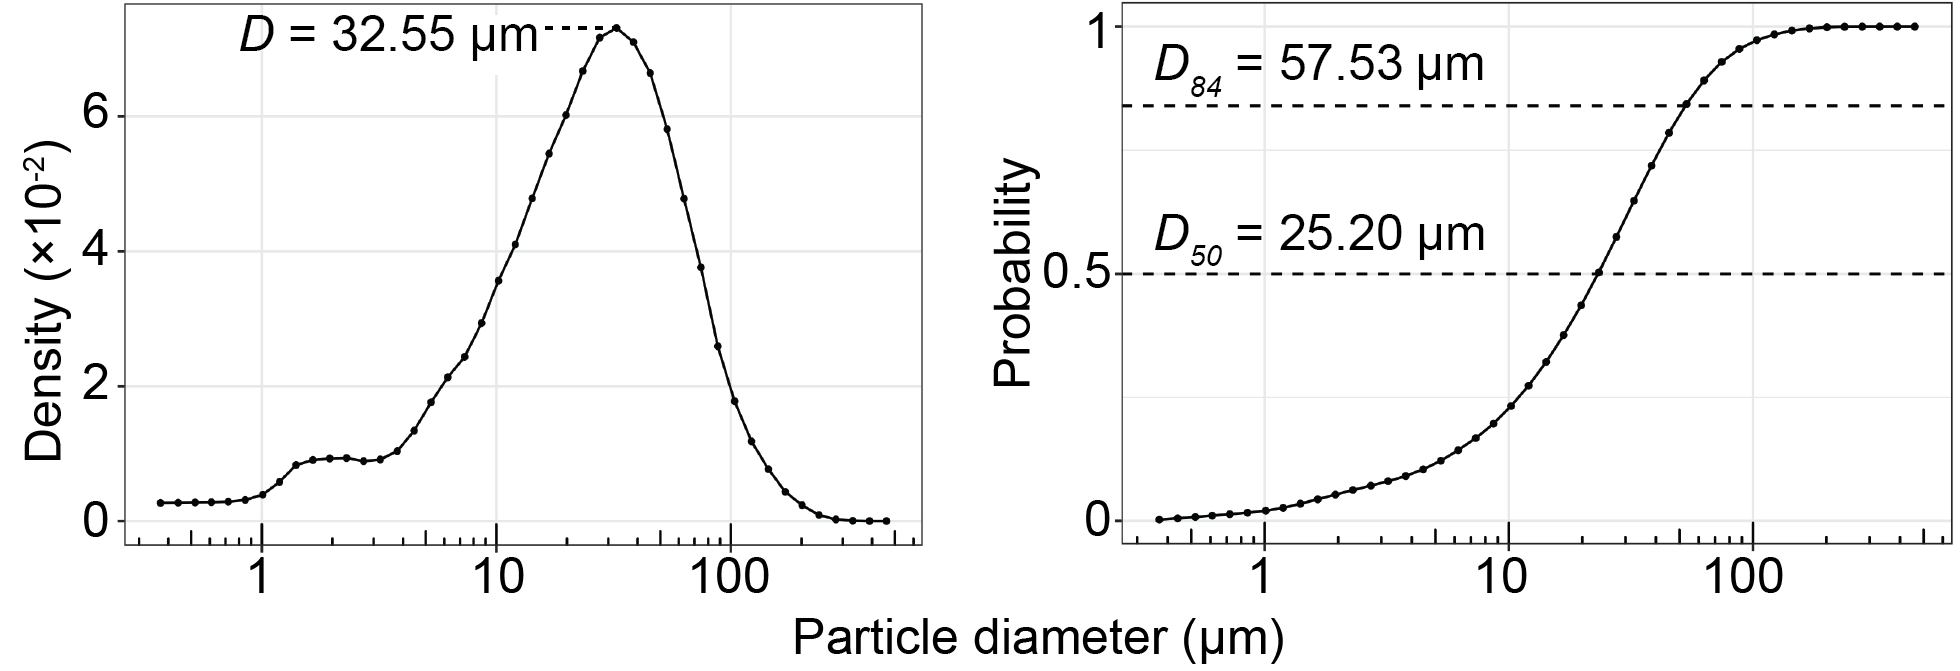
\includegraphics[width=15cm,trim = {0 3cm 0 0},clip]{wf5-200sizedist.png}
\centering
\caption{Particle size distribution of WF5-200 walnut shell flour used as sediment in experiments, expressed as a probability density function (left) and cumulative density function (right). The mode of the distribution (left) and the 50th and 84th percentiles (right) are labeled.}
\label{fig:sedsize}
\end{figure}

\subsection{Particle Concentration Run Protocols}

\subsection{Flow Characterization Run Protocols}

\section{Statistical Analysis}

\chapter{Results}

TODO

\chapter{Discussion}

TODO

The assumption that probability of retention (\(p_r\)) is 100\% when stems are coated with grease might be questionable based on our result that biofilm increased \(\eta\prime\) in comparison to greased dowels. The only other effect of biofilm that is readily apparent to me is perhaps increasing effective stem diameter (\(d_c\)). However, with our model for Reynolds number (\(\Rey_c \propto d_c\)), and both us and \citet{Fauria_2015} finding \(\eta\prime \sim -\Rey_c\), increasing stem diameter would be expected to have the opposite effect, unless I'm missing something.

\bibliographystyle{apalike}
\bibliography{refs}

\end{document}
